\section{Gaussian Process Regression}
\label{sec:overviewofgaussianprocessregression}

\subsection{Technical Overview}
\label{sub:technicaloverview}

The \ac{GP} can be used for nonparametric regression as follows: let $t_n$ be
the $n$th label observed in a series of noise-corrupted true target
variables $y_n$:
\begin{align*}
  t_n = y_n + \epsilon_n
\end{align*}
where $\epsilon_n \sim \mathcal{N}(0, \beta^{-1})$.  Then, the conditional distribution of
${\bf t} = [t_1, \dots, t_n]^\top$ given ${\bf y} =  [y_1, \dots, y_n]^\top$ follows
another Gaussian distribution of the form
\begin{align*}
  p ({\bf t} | {\bf y}) = \mathcal{N}({\bf t}| {\bf y}, \beta^{-1} \mat{I}_{N \times N}).
\end{align*}
The \ac{GP} then estimates the value of $y_n$ by computing the density $p({\bf t})$.
Using the definition of a \ac{GP}, the distribution over ${\bf t}$ is a zero-mean Gaussian
distribution with covariance given by a Gram matrix $\mat{K}$:
\begin{align*}
  p ({\bf y}) = \mathcal{N} ({\bf y}| {\bf 0}, \mat{K}).
\end{align*}
The Gram matrix encodes the correlation between two $M$-dimensional training inputs, ${\bf
  x}_i$ and ${\bf x}_j$.  This correlation can be computed from any function that
satisfies the properties of a kernel function, $k(\cdot,
\cdot)$~\cite{aizerman1964theoretical}.  Using the law of total probability and expanding
the Gaussian pdf:
\begin{align}
  \label{eqn:cov}
  p({\bf t}) &= \int p({\bf t} | {\bf y}) p({\bf y}) d {\bf y} \notag \\
  &= \mathcal{N}({\bf t}|{\bf 0}, \mat{C}),
\end{align}
where $C({\bf x}_i, {\bf x}_j) = k({\bf x}_i, {\bf x}_j) + \beta^{-1} \delta_{ij},$ and
$\delta_{ij}$ is the discrete impulse function.

Given a test input, ${\bf x}_{N+1}$, let joint distribution of $t_1, \dots, t_{N+1}$ is a
zero-mean Gaussian with covariance $\mat{C}_{N+1}$ given by
\begin{align*}
  \mat{C}_{N+1} &= \begin{bmatrix}
    \mat{C}_N & {\bf k} \\
    {\bf k}^\top & c \\
  \end{bmatrix},
\end{align*}
where $\mat{C}_N$ is the covariance function from Equation \ref{eqn:cov}, ${\bf k} \in
\mathbb{R}^N$ contains the values of $k({\bf x}_n, {\bf x}_{N+1}), n = 1,\dots,N$, and $c
= k({\bf x}_{N+1}, {\bf x}_{N+1}) + \beta^{-1}$.  Using well-known properties of Gaussian
distributions, we can express the conditional density $p(t_{N+1} | {\bf t})$ as having
mean and variance:
\begin{align*}
% \label{eqn:meanCov}
  \mu ({\bf x}_{N+1}) &= {\bf k}^\top \mat{C}_N^{-1} {\bf t} \notag \\
  \sigma^2({\bf x}_{N+1}) &= c - {\bf k}^\top \mat{C}_N^{-1} {\bf k}.
\end{align*}
Therefore the \ac{GP} has the nice property that besides computing a regression using
$\mu(\cdot)$, it also establishes a confidence region using the value of
$\sigma^2(\cdot)$.

\subsection{Learning Kernel Hyperparameters}
\label{sub:learningkernelhyperparameters}

The kernel function $k(\cdot, \cdot)$, described in \secref{sub:technicaloverview},
typically has a set of associated hyperparameters, ${\boldsymbol \Theta}$.
To ``learn'' a \ac{GP} is to find the value of ${\boldsymbol \Theta}$ that
minimizes the negative log-likelihood function:
\begin{align*}
  -\ln p({\bf t} | {\boldsymbol \Theta}) &= \frac{1}{2} \ln | \mat{C}_N | + \frac{1}{2}
  {\bf t}^\top \mat{C}_N^{-1} {\bf t} + \frac{N}{2} \ln (2\pi)
\end{align*}
Typically, to minimize this function one uses gradient descent.  The partial derivatives
for the $i$th hyperparameter is given by the following expression:
\begin{align}
  \label{eqn:learn}
  -\frac{\partial}{\partial {\Theta}_i} \ln p({\bf t} | { \Theta})
  &= \frac{1}{2} \text{trace} \left(\mat{C}_{N}^{-1} \frac{\partial \mat{C}_N}{\partial
      { \Theta}_i}\right) - \frac{1}{2} {\bf t}^\top \mat{C}_N^{-1}
  \frac{\partial \mat{C}_N}{\partial { \Theta}_i} \mat{C}_N^{-1} {\bf t}
\end{align}
These gradients may be evaluated symbolically if there exists an analytic solution, or
numerically otherwise.  For this project, we use the sparse kernels derived in the
\ac{ACFR} paper on the subject, to be covered in \secref{sub:exactlysparsekernels}.

Once the gradient has been computed, the $i$th hyperparameter in ${\boldsymbol \Theta}$
can be updated after the $k$th iteration of gradient descent algorithm as follows:
\begin{align*}
  { \Theta}_i^{k+1} \gets { \Theta}_i^k + \eta \frac{\partial}{\partial
    \Theta_i^{k}} \ln p({\bf t} | {\boldsymbol \Theta}),
\end{align*}
where $\eta$ is a learning parameter that for \ac{GP} regression is typically set to 0.1.
To overcome local-minima, learning a \ac{GP} typically involves using many initial guesses
of the hyperparameters, and picking the one that converges to a value that is most likely.

Figure~\ref{fig:learn} shows a toy example of the effect of choice of hyperparameters on
the log-likelihood.  The best choice of ${\boldsymbol \Theta}$ is the one that maximizes
the likelihood, or equivalently minimizes the negative log-likelihood as discussed above.

\begin{figure}[t]
  \begin{center}
    \subfigure[$\ln p({\bf t} | {\boldsymbol \Theta}) = 4.53$] {
      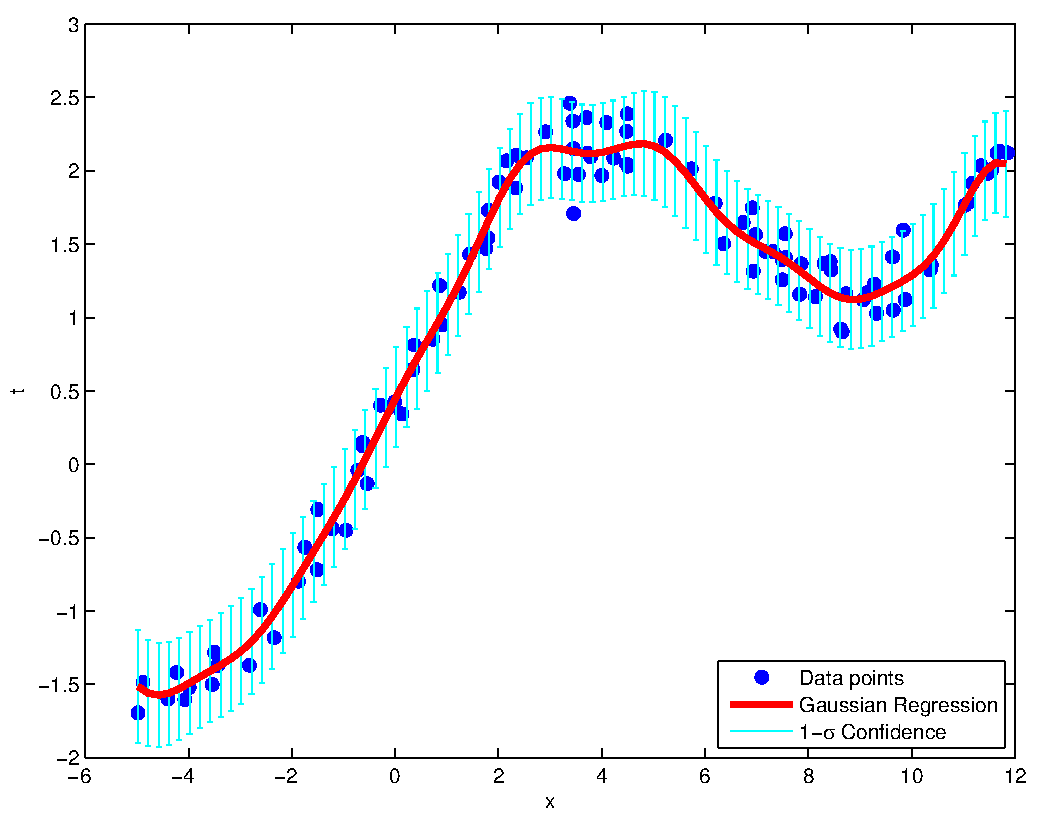
\includegraphics[width=0.38\columnwidth]{figures/problem3a_1_0_1}
      \label{fig:learn1}}
    \subfigure[$\ln p({\bf t} | {\boldsymbol \Theta}) = -80.44$] {
      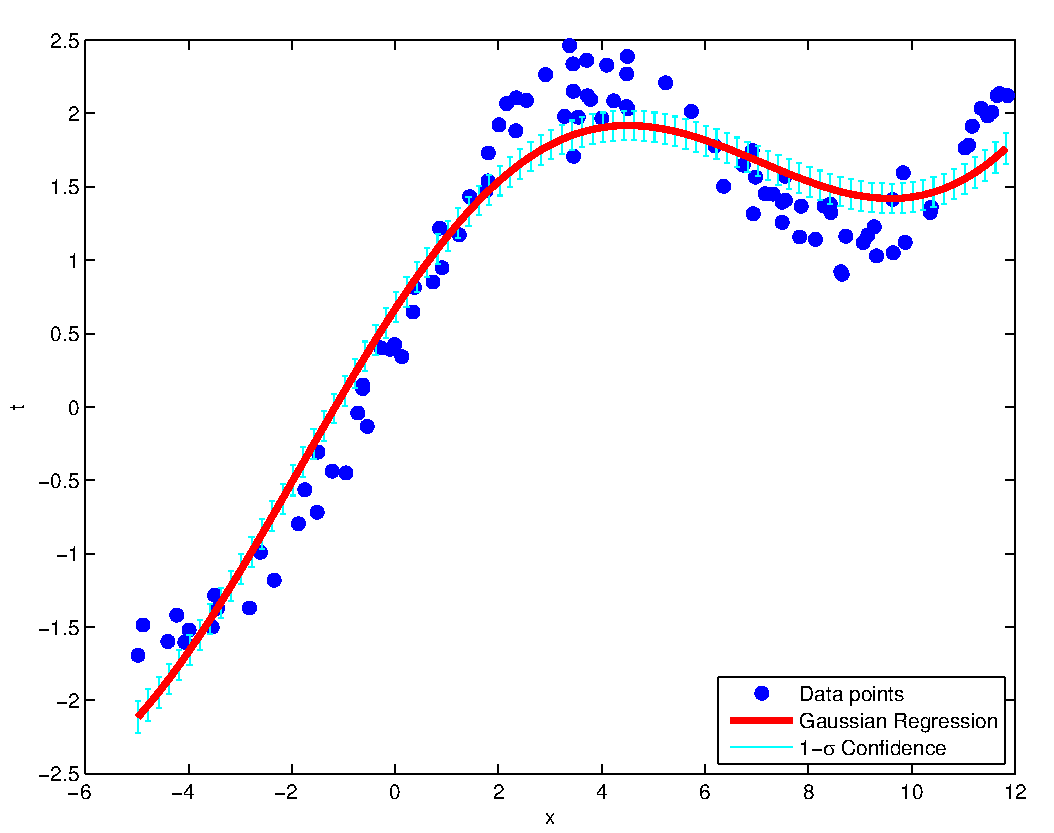
\includegraphics[width=0.38\columnwidth]{figures/problem3a_10_0_01}
      \label{fig:learn2}}
    \subfigure[$\ln p({\bf t} | {\boldsymbol \Theta}) = -133.89$] {
      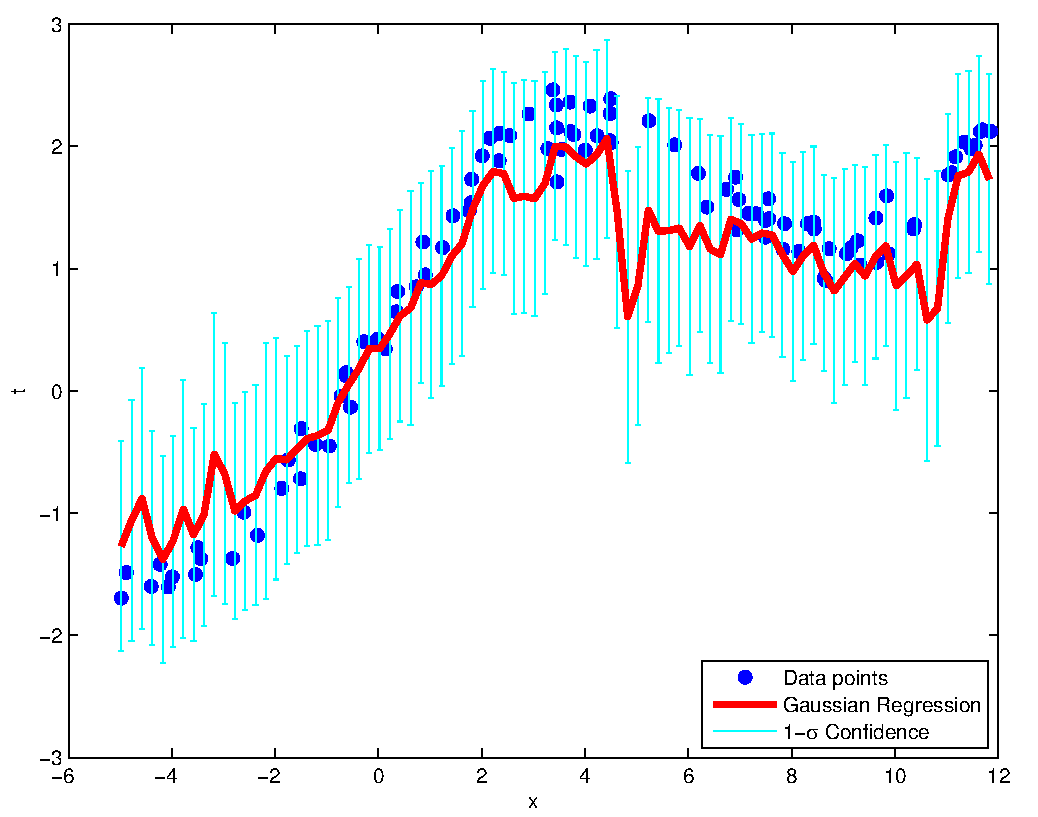
\includegraphics[width=0.38\columnwidth]{figures/problem3a_0_2_0_5}
      \label{fig:learn3}}
    \subfigure[$\ln p({\bf t} | {\boldsymbol \Theta}) = 16.33$] {
      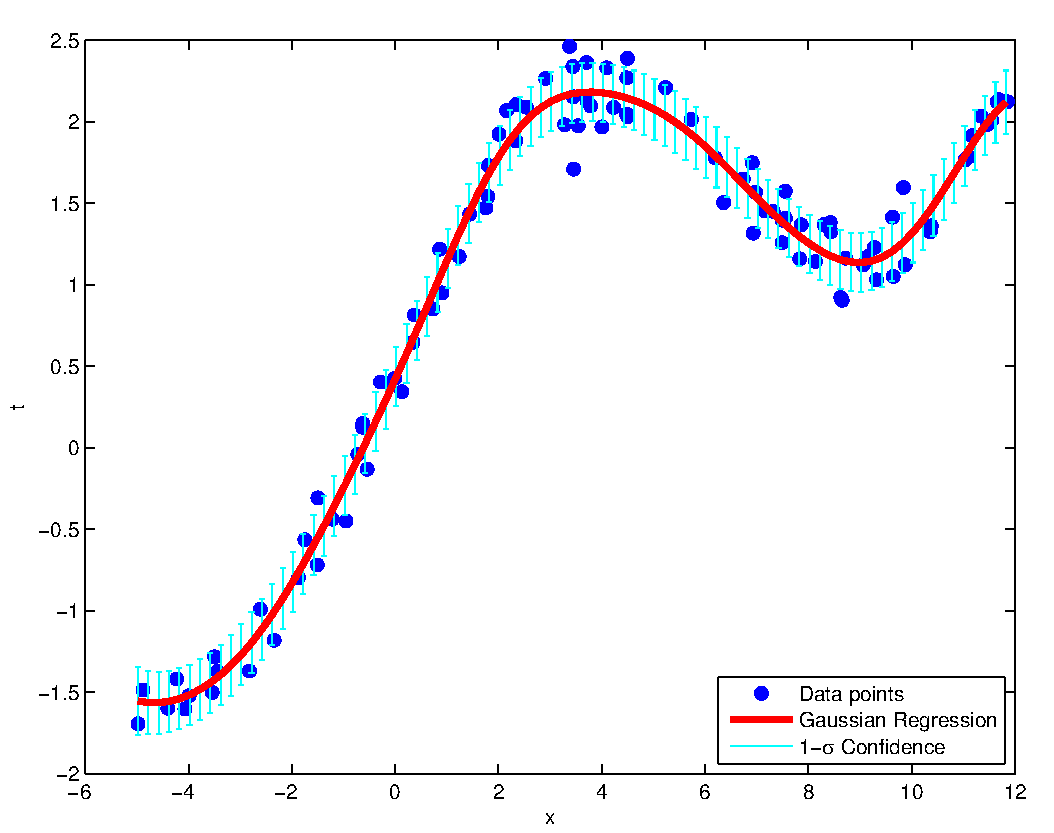
\includegraphics[width=0.38\columnwidth]{figures/problem4d}
      \label{fig:learn4}}
    \caption{ {\small Example of log-likelihood of various hyperparameters for a small
        \ac{GP} regression example using our C implementation of \ac{GP} regression for
        $N=100$, $M=1$.  In blue are the training points ${\bf x}_n$.  In red are the
        values of $\mu(\cdot)$ evaluated at various test points, and the 1-$\sigma$
        confidence intervals, computed from $\sigma^2(\cdot)$, are denoted in cyan.  In
        \subref{fig:learn1}, \subref{fig:learn2}, and \subref{fig:learn3}, the choices of
        hyperparameters do not maximize the log-likelihood function, $\ln p({\bf t} |
        {\boldsymbol \Theta})$.  In \subref{fig:learn4}, the optimal value of the
        hyperparameters was found using gradient descent, which maximizes the
        likelihood.} }
    \label{fig:learn}
  \end{center}
\end{figure}

\subsection{High-level Considerations for Parallel Implementation}
\label{sub:considerationsforparallelimplementation}

The two most important computational steps in \ac{GP} are taken from
Equations~\ref{eqn:cov} and \ref{eqn:learn}.  For the considerations in this report,
we do not resort to clustering the training data as is typically done in related work.
Instead, we consider how to achieve parallelism using iterative solvers.

Starting with Equation~\ref{eqn:cov}, it is clear that storing the covariance matrix
$\mat{C}_N$ is, in general, infeasible for large datasets due to memory limitations.
Therefore, the kernel function ought to be sparse to make \ac{GP} regression feasible in
this case.  This will be discussed further in \secref{sub:exactlysparsekernels}.

In order to evaluate $\mu(\cdot)$ and $\sigma^2(\cdot)$, one must solve the linear systems
$\mat{C}_N {\bf x} = {\bf t}$ and $\mat{C}_N {\bf x} = {\bf k}$, respectively (where ${\bf
  x}$ denotes the solution vector).  Unsurprisingly, the inverse of $\mat{C}_N$ will be
dense even if $\mat{C}_N$ is sparse, and it is much more computationally efficient to solve
these linear systems than to actually multiply by the stored inverse.

The procedure of learning the hyperparameters, summarized in Equation~\ref{eqn:learn}, is
more complicated than inference.  To compute the second term, one must first
solve the linear system $\mat{C}_N {\bf x} = {\bf t}$, followed by solving the system
$\mat{C}_N {\bf x}' = {\bf x}$, and compute the inner product of ${\bf t}$ and ${\bf x}'$.

Computing the first term in Equation~\ref{eqn:learn} is somewhat computationally expensive
because the inverse of $\mat{C}_N$ can not be stored.  Thus to compute this term, we must
solve $N$ linear systems for the $N$ columns of $\frac{\partial \mat{C}_N}{\partial
  {\boldsymbol \Theta}_i}$.  Then, the trace is simply the sum of the $i$th elements of
the solution vector for $i = 1,\dots,N$.  See \secref{sec:implementation} for the details
of how this is acheived with \ac{MPI}.

The steps mentioned above call for solving many linear systems of the form $\mat{A} {\bf
  x} = {\bf b}$, where $\mat{A}$ is \ac{PD}.  Though typically Cholesky decomposition is
done when $\mat{A}$ is small, as A gets very large (say, $\mat{A} \in \mathbb{R}^{10^6
  \times 10^6}$) direct solvers, such as Cholesky decomposition, were quite slow in our
initial implementation of \ac{GP} regression, even when using the GPU-enabled SuiteSparse
package for Cholesky-based solvers.  This is because the computational complexity of
Cholesky decomposition is $O(n^3)$.

\begin{figure}[t]
  \begin{center}
    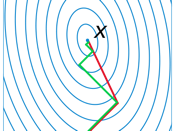
\includegraphics[width=0.3\textwidth]{figures/cg}
    \caption{{\small The conjugate gradient method (red) typically has faster convergence
      properties than standard gradient descent (green), and works well on large matrices
      where Cholesky Decomposition is too computationally expensive.  The minima is
      denoted by {\bf x}, and the contours of the nonlinear function are shown in blue.
      In this example the conjugate gradient converges in only two iterations, compared
      to the six iterations taken by gradient descent.}}
    \label{fig:cg}
  \end{center}
\end{figure}

Instead, we use sparse iterative solvers to acheive parallelism.  In particular, we use
the \ac{KSP}-type method (conjugate gradient descent) with a Jacobi preconditioner.  This
approach is a well-known alternative to Cholesky decomposition~\cite{hestenes1952methods},
and a visual comparison to gradient descent is shown in Figure~\ref{fig:cg}\footnote{This
  figure was taken from
  \texttt{http://en.wikipedia.org/wiki/Conjugate\_gradient\_method}}.  Routines for
\ac{KSP} solvers are available from the Argonne National Laboratory's \ac{PETSc}
package~\cite{petsc-efficient, petsc-user-ref, petsc-web-page}.

\subsection{Exactly Sparse Kernels}
\label{sub:exactlysparsekernels}

We will call the two kernels $k_1(\cdot, \cdot)$ and $k_2(\cdot, \cdot)$ discussed
in~\cite{melkumyan2009sparse} as the ``Type 1'' and ``Type 2'' kernels, respectively.
These kernels are desirable for this project because both are sparse and both have
analytic expressions for the partial derivatives of the likelihood for each of their
hyperparameters.

In the following sections, we enumerate the definitions of the kernels and expressions for
the partial derivatives of the log-likelihood functions.  Figure~\ref{fig:dist} provides a
simple visualization for the underlying metric spaces used for each kernel.

\begin{figure}[t]
  \begin{center}
    \subfigure[Product of Absolute Distances] {
      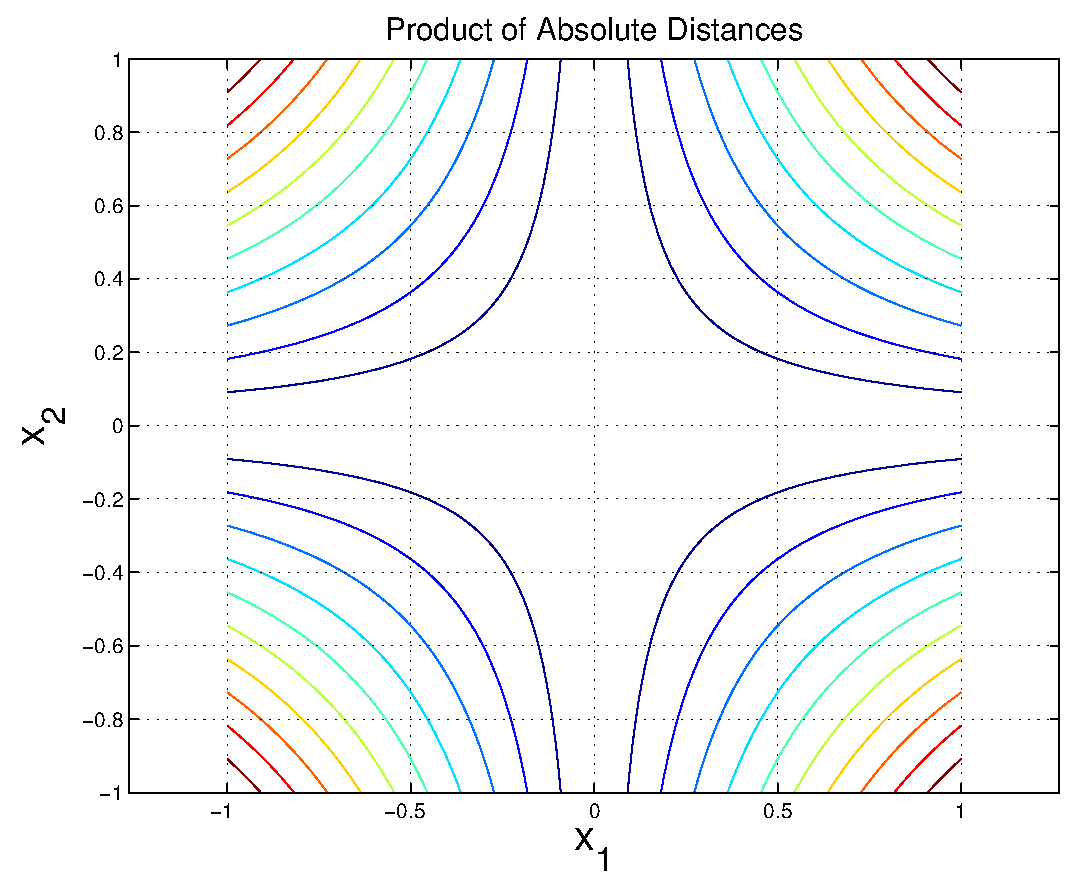
\includegraphics[width=0.38\columnwidth]{figures/pad}
      \label{fig:dist:pad}}
    \subfigure[Mahalanobis Distances] {
      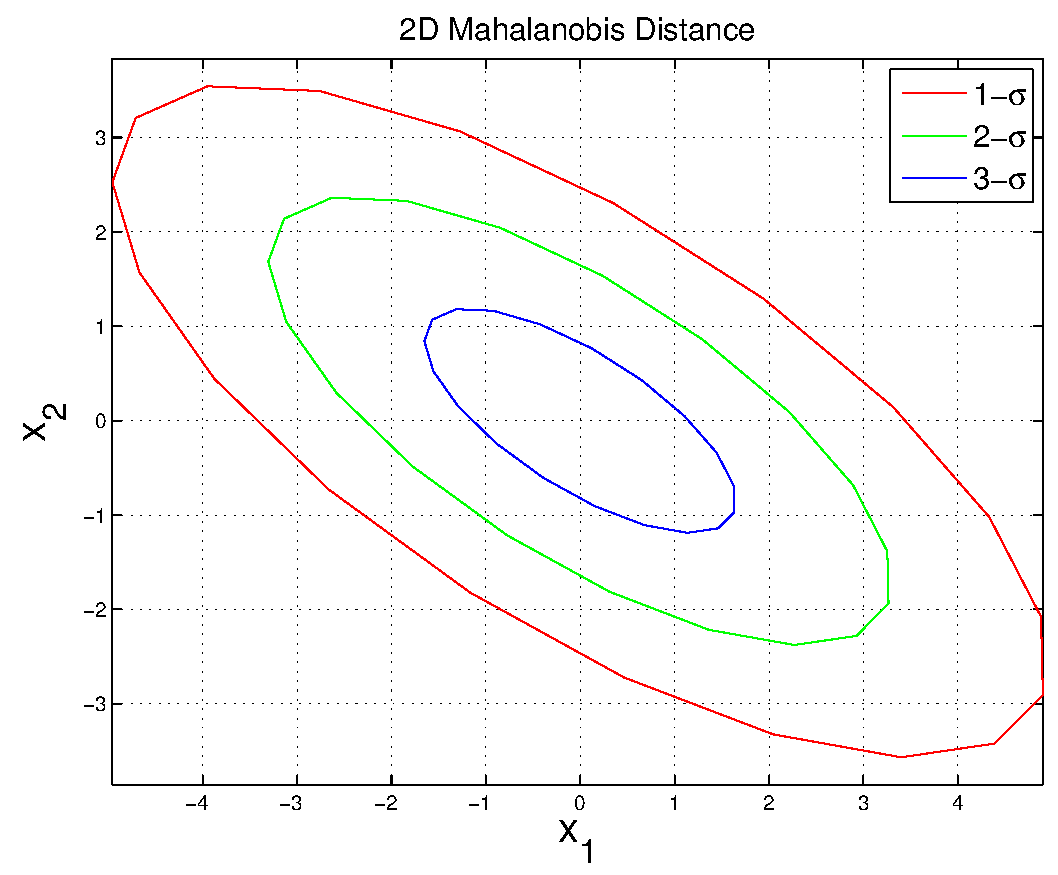
\includegraphics[width=0.38\columnwidth]{figures/mahal}
      \label{fig:dist:mahal}}
    \caption{A visualization of the underlying metric spaces used in the kernels
      from~\cite{melkumyan2009sparse} when $M=2$.  Each contour represents the points
      which have the same distance from the origin.  In \subref{fig:dist:pad}, the
      distance between two training points is based on a product of absolute distances.
      In \subref{fig:dist:mahal}, the distance is statistically motivated by the Gaussian
      distribution; in this plot there is some correlation in the 2$\times$2 covariance
      matrix $\Omega^{-1}$, however, in computing the gradient of the likelihood we assume
      zero correlation.}
    \label{fig:dist}
  \end{center}
\end{figure}

\subsubsection{ACFR Kernel Type 1}
\label{subs:acfrkerneltype1}

First let us consider the 1D case, where $M = 1$.  The hyperparameters for the ACFR Type 1
kernel are ${\boldsymbol \Theta} = \begin{bmatrix}
    \sigma_0 & l
  \end{bmatrix}^\top $. For two 1D training points, $x$ and $x'$, the kernel is defined as
\begin{align*}
  k_1 (x, x'; \sigma_0, l) &= \left\{
    \begin{array}{cc}
      \sigma_0 \left[\frac{2+\cos(2\pi \frac{d}{l})}{3} \left(1 -
          \frac{d}{l}\right) + \frac{1}{2\pi} \sin \left(2\pi \frac{d}{l}\right)\right] \ \
      & \text{if}\ \ d < l \\
      0, & \text{if}\ \ d \ge l
    \end{array}
  \right.,
\end{align*}
where $d = |x - x'|$.  For arbitrary $M$, the kernel is given by
\begin{align*}
  k^{(M)}_1 ({\bf x}, {\bf x}'; {\bf l}, \sigma_0) &= \sigma_0 \prod\limits_{i=1}^{M} k_1
  (x_i, x_i'; l_i, 1).
\end{align*}

The partial derivatives of the kernel are as follows:
\begin{align*}
  \frac{\partial k_1^{(M)}}{\partial
    \sigma_0} &= \frac{1}{\sigma_0} k_1^{(M)} \\
  \frac{\partial k_1^{(M)}}{\partial
    l_i} &= \left\{
    \begin{array}{cc}
      \frac{4\sigma_0}{3} \frac{d_i}{l_i^2} \left[\pi \left(1 - \frac{d_i}{l_i}\right)
        \cos \left(\pi \frac{d_i}{l_i}\right) + \sin \left(\pi \frac{d_i}{l_i}\right)\right]
      \sin \left(\pi \frac{d_i}{l_i}\right) & \text{if}\ \ d_i < l_i \\
      0, & \text{if}\ \ d_i \ge l_i
    \end{array}
  \right.
\end{align*}

\subsubsection{ACFR Kernel Type 2}
\label{subs:acfrkerneltype2}

The ACFR Type 2 kernel is equivalent to the Type 1 kernel when $M = 1$.  For arbitrary
$M$,
\begin{align*}
  k_2^{(M)} (r; \sigma_0, \Omega) &= \left\{
    \begin{array}{cc}
      \sigma_0 \left[\frac{2+\cos(2\pi r)}{3} \left(1 -
          r\right) + \frac{1}{2\pi} \sin \left(2\pi r\right)\right] \ \
      & \text{if}\ \ r < 1 \\
      0, & \text{if}\ \ r \ge 1
    \end{array}
  \right..
\end{align*}
where $r = \sqrt{({\bf x} - {\bf x}')^\top \Omega ({\bf x} - {\bf x}')}$ is the
Mahalanobis distance for information matrix $\Omega$, which for uncorrelated features we
assume to be
\begin{align*}
  \Omega &= \text{diag}\left(\frac{1}{l_1^2}, \dots, \frac{1}{l_M^2}\right).
\end{align*}
Under this assumption, the partial derivatives are
\begin{align*}
  \frac{\partial k_2^{(M)}}{\partial
    \sigma_0} &= \frac{2+\cos(2\pi r)}{3} (1 - r) + \frac{1}{2\pi} \sin (2\pi r), \ 
  \ \text{if}\ \ 0 \le r < 1 \\
  \frac{\partial k_2^{(M)}}{\partial
    l_i} &= \frac{4\sigma_0}{3} \frac{1}{l_i} \left[\pi \left(1 - r\right)
        \cos \left(\pi r\right) + \sin \left(\pi r\right)\right]
      \frac{\sin \left(\pi r\right)}{r} \left(\frac{x_i - x_i'}{l_j}\right)^2 \text{if}\ \
      0 < r < 1.
\end{align*}
If $r\ge 1$, the gradient is always zero.  In the limit as $r \rightarrow 0$, then $
\frac{\partial k_2^{(M)}}{\partial l_i} = 0$.

%%% Local Variables: 
%%% mode: latex
%%% TeX-master: "../report.tex"
%%% End: 
